\chapter{Highway traffic in Czech Republic}

In order to be able to test platooning effects on real data of highway traffic in the Czech Republic we needed to take information about level of traffic statistics at different times in day and on different days in week, ration between passenger vehicles and trucks in highway, average speed and speed dispersion on highway. There is not a complex study which would provide us such information so we had to use some different resources and join them. We had to combine three sources of statistics and traffic models:

\begin{itemize}
\item Source 1:	Vysoké Mýto –  dopravní model a analýza dopravních proudů (Vysoke Myto – traffic model and analysis of traffic streams) Made by Moot MacDonald CZ, s.r.o. for Vysoke Myto council, published in January 2015\footnote{\url{http://projekty.vysoke-myto.cz/index.php/strategicke-dokumenty/dopravni-pruzkum}}.
\item Source 2:	Traffic statistics from tunnel Lochkov, Prague circuit – May 2014, received from ŘSD Praha – cannot be published
\item Source 3:	Traffic statistics of highway D1 published by ŘSD Praha in 2012\footnote{\url{http://www.ceskedalnice.cz/prilohy/intenzity-2012.pdf}}\footnote{\url{ttp://www.ceskedalnice.cz/odborne-info/intenzity-dopravy}}.
\end{itemize}










\section{Daily statistic and traffic structure }

The daily statistics are taken from Source 1 (Vysoke Myto) because it is a detail analysis. It was made on main route R35 that connects Bohemia and Moravia (Hradec Kralove – Olomouc) where there is no possibility to use a highway. All transit and local transport goes through this measured point and therefore the distributions of vehicle types and traffic density are similar to highway ones.


\begin{figure}[ph]
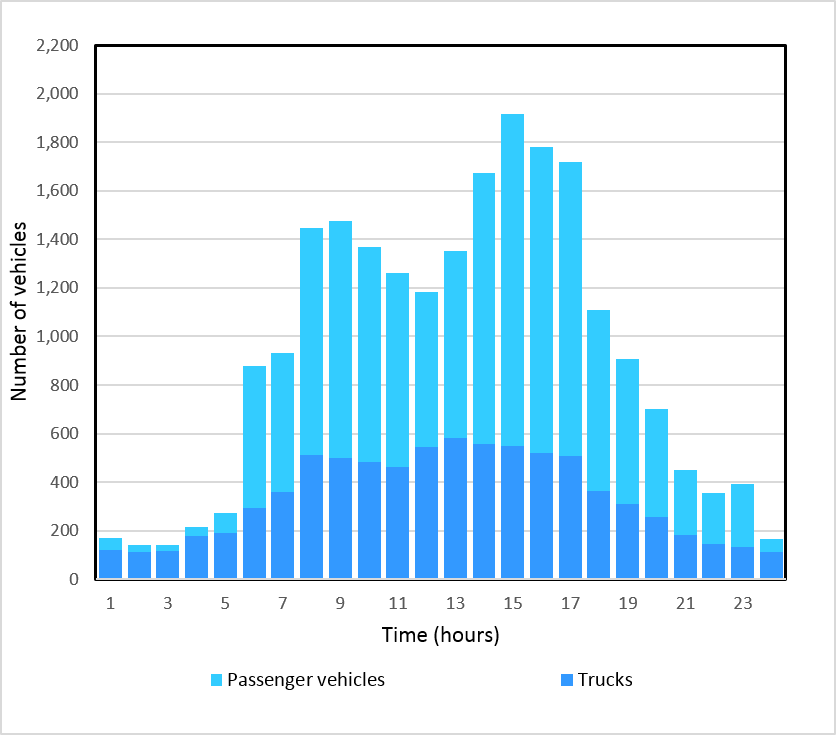
\includegraphics[width=0.90\textwidth,height=0.90\textheight,keepaspectratio]{figures/Chapter_2/2_Cum_diag_traffic_VM.png}
\centering
\protect\caption{\label{fig:2_1-1}Cumulative diagram of number of passenger vehicles plus number of trucks per hour during a day in Vysoke Myto}
\end{figure}

There are results of traffic monitoring which was made in Vysoke Myto in September 2014 in the Figure \ref{fig:2_1-1}. You can see that there are two  rush hours in a day (morning 7-10, 14-17 o'clock). The ratio passenger vehicles and trucks change in day, there are fewer cars in night hours and during day the number of cars increases and it is nearly double of trucks  as you can see in Table \ref{tab:2_1-1}.

\begin{table}
\begin{centering}
\begin{tabular}{|c|c|c|c|c|c|c|c|c|c|}
\hline 
Hours & 1:00 & 2:00 & 3:00 & 4:00 & 5:00 & 6:00 & 7:00 & 8:00  \tabularnewline
\hline 
Cars in traffic & 30\% & 21\% & 17\% & 16\% & 30\% & 67\% & 62\% & 65\%  \tabularnewline
\hline 
 &  &  &  &  &  &  &  &  \tabularnewline
\hline 
Hours & 9:00 & 10:00 & 11:00 & 12:00  & 13:00 & 14:00 & 15:00 & 16:00\tabularnewline
\hline 
Cars in traffic & 66\% & 65\% & 63\% & 54\% & 57\% & 67\% & 71\% & 71\%\tabularnewline
\hline 
 &  &  &  &  &  &  &  &  \tabularnewline
\hline 
Hours & 17:00 & 18:00 & 19:00 & 20:00 & 21:00 & 22:00 & 23:00 & 24:00\tabularnewline
\hline 
Cars in traffic & 70\% & 67\% & 66\% & 63\% & 59\% & 59\% & 66\% & 32\%\tabularnewline
\hline 
\end{tabular}
\centering
\protect\caption{\label{tab:2_1-1}Percentages of passenger vehicles in all traffic during a day}
\end{centering}
\end{table}

\section{Monthly statistic of cumulative quantity of vehicles}

For this statistic we decided to use Source 2 (tunnel Lochkov). In Figure \ref{fig:2_2-1} there is cumulative number of vehicles for both directions in May 2014. By this analysis we wanted to show, that the traffic distribution repeats  weekly and the level of traffic depends on working and weekend days.

\begin{figure}[ph]
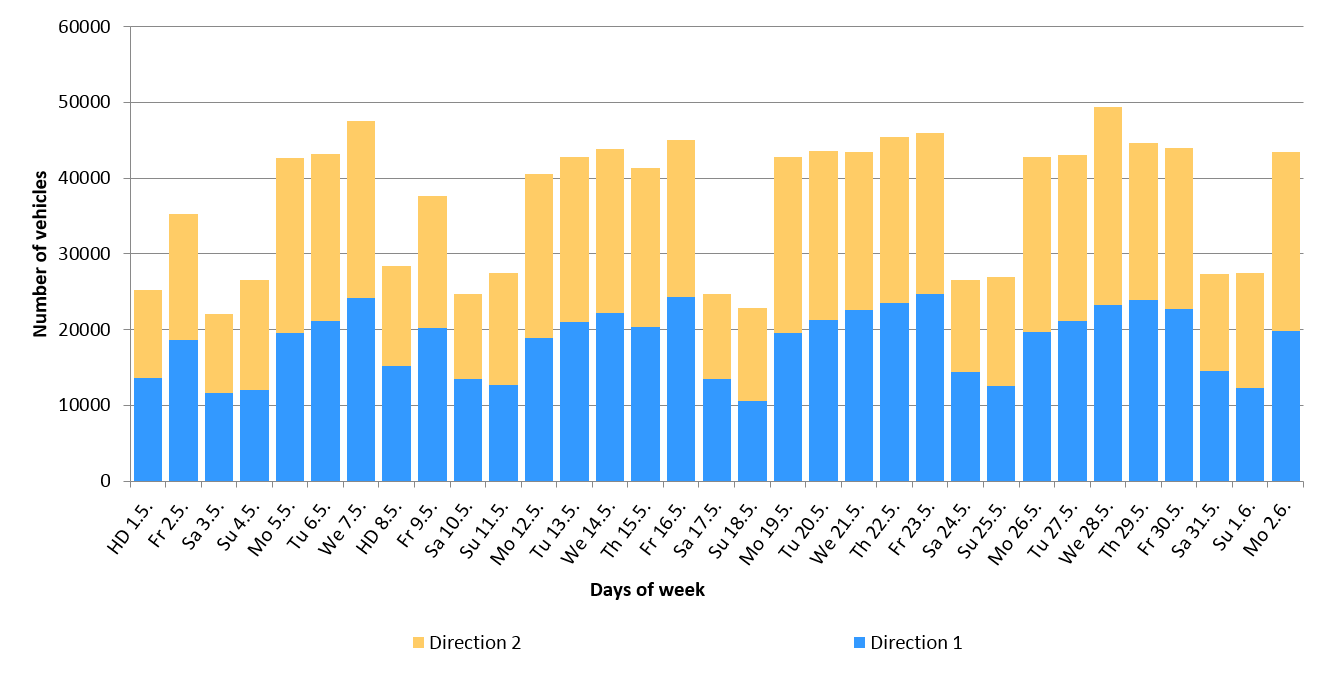
\includegraphics[width=0.85\textwidth,height=0.90\textheight,keepaspectratio]{figures/Chapter_2/2_Cum_diag_month.png}
\centering
\protect\caption{\label{fig:2_2-1}Cumulative diagram of number of traffic in both directions per day during May}
\end{figure}

In this monthly statistics (Figure \ref{fig:2_2-1}) you can see that traffic density is influenced by work days in week. On weekends the traffic density is about a half of work days density. In May 2014 there were two holidays during week (Thursday 1.5. and Thursday 8.5. in 2014) and you can see low traffic density too on these days, and even on the following Fridays the density is lower than on other Fridays.





  
  
  
  


\section{Number of vehicles per day in highway}

For this statistics we decided to use Source 3 (highway D1) where average number of vehicles per day is recorded in both directions in several parts of highway D1. See example in Table \ref{tab:2_3-1}. According to the data we can also say that in last several years there was no big increase of volume of traffic. So we can expect that the number of vehicles per day in year 2015 should be similar to the numbers in year 2012.

\begin{table}[ph]
\begin{centering}
\begin{tabular}{|c|c|c|c|c|c|c|}
\hline 
Part of D1 / Year & 1994 & 2000 & 2006 & 2008 & 2010 &  2012\tabularnewline
\hline 
Spořilov – Chodov & 47 700 &	71 400 &	94 900 &	98 200 &	88 800 &	90700\tabularnewline
\hline 
Chodov - Průhonice &	35 700 &	62 600 &	- &	91 900 &	82 500 &	84400\tabularnewline
\hline 
Soutice - Loket &	18 000 &	26 200 &	35 700 &	37 700 &	37 000 &	37000\tabularnewline
\hline 
Devět Křížu - Ostrov. &	20 400 &	35 800 &	39 100 &	41 300 &	41 200 &	41300\tabularnewline
\hline 
Ostrovačice - Kývadla &	20 900 &	36 700 &	39 900 &	- &	42 900 &	43100\tabularnewline
\hline 
\end{tabular}
\centering
\protect\caption{\label{tab:2_3-1}Number of vehicles which go though a part of highway D1 per day in both directions}
\end{centering}
\end{table}











\section{Speeds in highway}

For the maximum usage of highway it is expected to drive by maximum speed which is in the Czech Republic 130 km/h , it is about 36 m/s. For the simulator, Chapter 4, which increase the vehicle speed by 1 m/s in changing of lane, we set that average speed in 34 m/s. So in three-lane highway the average speed is not higher than speed limit.

We used speed dispersion of 3m/s to create various vehicles in highway, no two drivers go at the same speed.







\section{Model situations for simulation}

In order to make the future testing easier, we set some traffic model situations.


\subsection*{Traffic model \#1 – part of D1: Chodov – Průhonice}

This part of highway D1 was chosen as a three-lane highway which corresponds to classic example of highway entrance to a big city. We chose time 14:00 that is rush hour in highway and set modelling conditions in Table  \ref{tab:2_5_1-1} according Figure \ref{fig:2_5_1-1} for 42 200 vehicles per day (Table \ref{tab:2_3-1}) in one direction.

\begin{table}[ph]
\begin{centering}
\begin{tabular}{|c|c|}
\hline 
Number of vehicles per hour in one lane &	3 200\tabularnewline
\hline 
Average speed &	34 m/s\tabularnewline
\hline 
Speed dispersion &	3m/s\tabularnewline
\hline 
Percentage of passenger vehicles in traffic & 	67\%\tabularnewline
\hline 
Trucks speed &	25 m/s\tabularnewline
\hline 
Number of lanes in highway &	3\tabularnewline
\hline 
\end{tabular}
\centering
\protect\caption{\label{tab:2_5_1-1}Features of Traffic model \#1}
\end{centering}
\end{table}


\begin{figure}[ph]
\begin{centering}
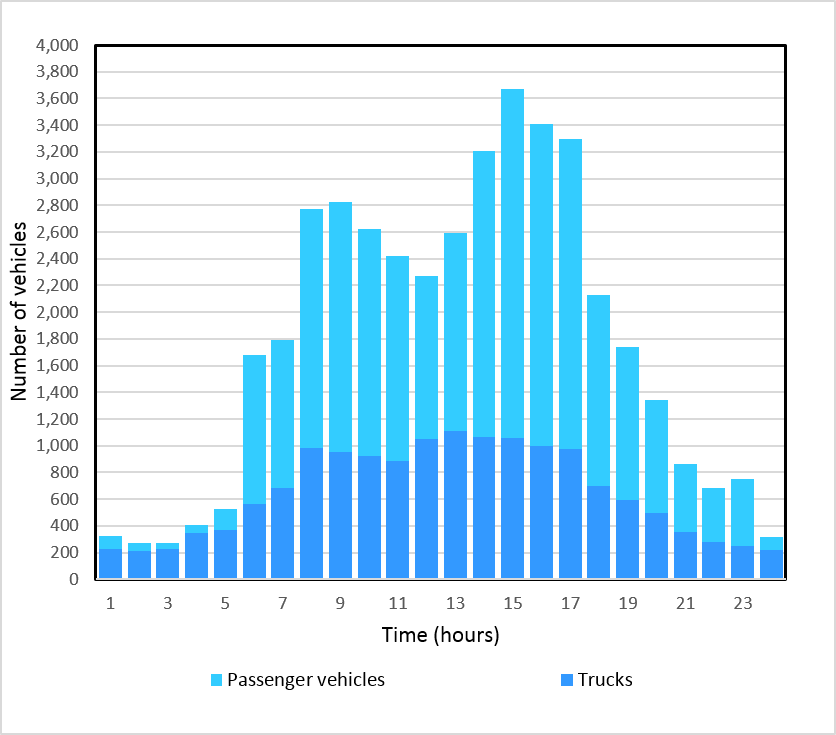
\includegraphics[width=0.60\textwidth,height=0.60\textheight,keepaspectratio]{figures/Chapter_2/2_Cum_diag_day_42200.png}
\centering
\protect\caption{\label{fig:2_5_1-1}Cumulative diagram of number of passenger vehicles plus number of trucks per hour for 42 200 vehicles per day}

\end{centering}
\end{figure}

\subsection*{Traffic model \#2 – Tunnel Lochkov}

We chose time 13:00 that is rush hour in highway (we wanted to test different than in Traffic model \#1) and set modelling conditions in Table  \ref{tab:2_5_2-1} according Figure \ref{fig:2_5_2-1} for 22 000 (average of workdays from Figure \ref{fig:2_2-1}) in one direction.

\begin{table}[ph]
\begin{centering}
\begin{tabular}{|c|c|}
\hline 
Number of vehicles per hour in one lane &	1 650\tabularnewline
\hline 
Average speed &	34 m/s\tabularnewline
\hline 
Speed dispersion &	3m/s\tabularnewline
\hline 
Percentage of passenger vehicles in traffic & 	67\%\tabularnewline
\hline 
Trucks speed &	25 m/s\tabularnewline
\hline 
Number of lanes in highway &	2\tabularnewline
\hline 
\end{tabular}
\centering
\protect\caption{\label{tab:2_5_2-1}Features of Traffic model \#2}
\end{centering}
\end{table}

\begin{figure}[ph]
\centering
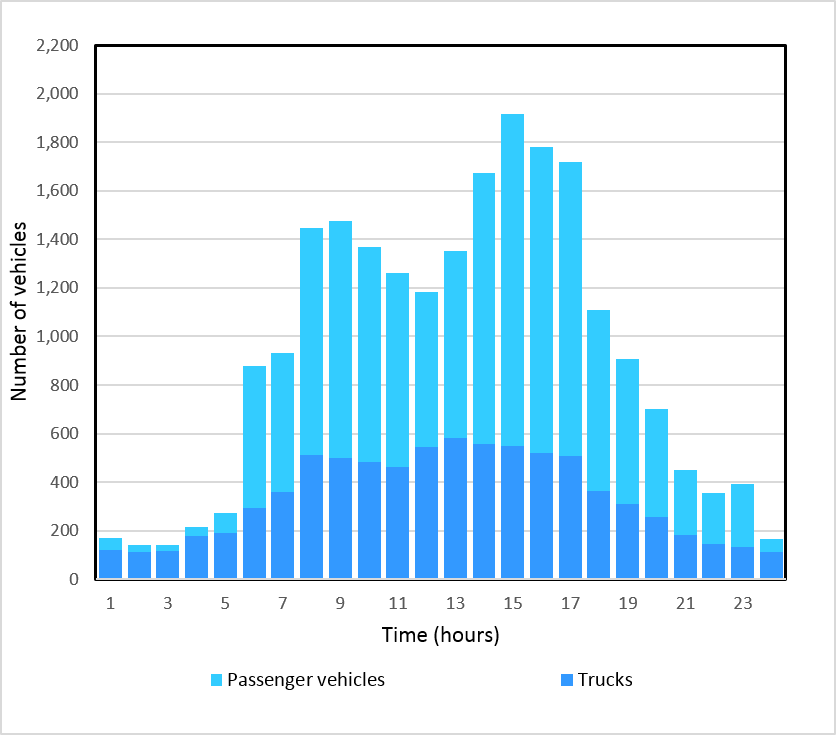
\includegraphics[width=0.60\textwidth,height=0.60\textheight,keepaspectratio]{figures/Chapter_2/2_Cum_diag_day_22000.png}
\centering
\protect\caption{\label{fig:2_5_2-1}Cumulative diagram of number of passenger vehicles plus number of trucks per hour for 22 200 vehicles per day}
\end{figure}